\begin{homeworkProblem}
  Reconstrucción de imágenes a partir de sus bordes.\\
  El operador laplaciano en $2D$ se define como:
  \begin{align*}
    \nabla^2 u(x,y)&=\frac{\partial u}{\partial x^2}+\frac{\partial u}{\partial y^2}
  \end{align*}
  donde $u(x,y)$ es una función que representa la intensidad de los pixeles de la imagen en el dominio espacial. El operador Laplaciano se utiliza para detectar bordes porque responde a las variaciones de la intensidad de los pixeles en la vecindad de cada punto. En áreas de la imagen donde la intensidad varia rapidamente (bordes), el Laplaciano tiene un valor alto, mientras que en áreas homogéneas (sin bordes) el Laplaciano es cercano a cero. El proceso de detección de bordes implica calcular el Laplaciano de la imagen $u(x,y)$, lo que da como resultado un mapa de bordes.\\
  En este ejercicio estamos interesados en reconstruir la imágen original $u(x,y)$ a partir de los bordes detectados.\\
  Para esto debemos resolver la ecuación de Poisson en $2D$
  \begin{equation}\label{eq:poisson}
    \nabla^2u(x,y)=f(x,y)
  \end{equation}
  donde $f(x,y)$ es el mapa de bordes.\\
  El problema \ref{eq:poisson} puede ser discretizado en un sistema de ecuaciones lineales de la forma:
  \begin{align*}
    Au=f
  \end{align*}
  donde $A$ es una matriz que representa el operador Laplaciano discreto, $u$ es el vector que contiene los valores de la imagen original en cada pixel (a reconstruir), y $f$ es el vector que contiene los valores de los bordes detectados.\\
  \begin{center}
    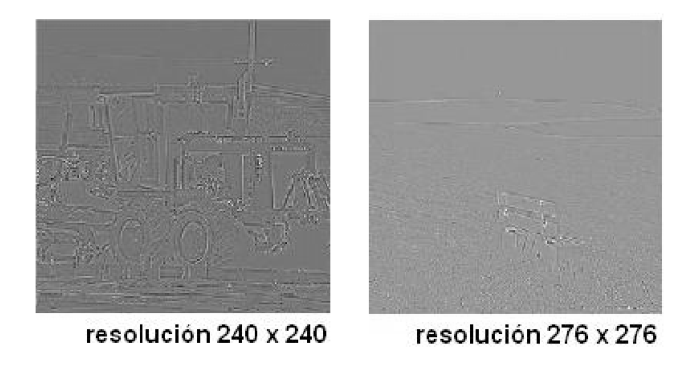
\includegraphics[scale=0.8]{Figures/imagenesproblema5.png}
  \end{center} 
  \textbf{Instrucciones:}\\
  Su tarea consiste en reconstruir las imágenes originales. En la pagina web del curso encuentran los archivos en Matlab bordes1.mat y bordes2.mat que contienen los datos de cada fotografía. Siga los pasos descritos a continuación:
  \begin{solucion}
    Usando la aproximación de diferencias finitas centrales para la segunda derivada:
    \begin{align*}
      \frac{\partial u}{\partial x^2}&\approx \frac{u_{i+1,j}-2u_{i,j}+u_{i-1,j}}{h^2},\\
      \frac{\partial u}{\partial y^2}&\approx \frac{u_{i,j+1}-2u_{i,j}+u_{i,j-1}}{h^2}.
    \end{align*}
    Sumando ambas expresiones obtenemos:
    \begin{align*}
      \frac{u_{i+1,j}+u_{i-1,j}+u_{i,j+1}+u_{i,j-1}-4u_{i,j}}{h^2}=f_{i,j}
    \end{align*}
    lo que nos ayudará a construir la matriz $A$ en el ejercicio.\\
    \textbf{Nota:} Profesor Mauricio, el tamaño de la matriz parece ser un gran problema para Matlab a la hora de calcular inversas en los métodos de Gauss-Seidel y SOR, por lo que nos fue necesaria buscar una forma de optimizar el proceso, a lo que decidimos investigar y encontrar una fuente en la que dan las fórmulas exactas de manera que "de alguna manera" optimiza el tiempo de o al menos facilita a matlab en el cálculo de los valores, dejamos la cita de la información a la que nos referimos \href{https://github.com/reece-iriye/Solving-2D-Poissons-Equation-Using-Finite-Difference-Method-and-Iterative-Solvers/tree/main}{Solving-2D-Poissons-Equation-Using-Finite-Difference-Method-and-Iterative-Solvers}, esperamos entienda la situación, de lo contrario simplemente usábamos el código que usamos en Jacobi modificando las $T$ y las $c$.
    Ahora veamos esto en la practica, daremos $100$ iteraciones a cada método y daremos el tiempo tomado para ejecutarse.\\
    Siendo así, a continuación dejaremos los códigos y las gráficas generadas.
    \newpage
    \begin{enumerate}
      \item Imágen 1 (Jacobi) $\frac{137}{4514}s\approx 0.0304 s$.
        \begin{lstlisting}[language = matlab]
format rational
%% Construcción de la matriz A usando diferencias finitas
function A = construir_matriz_A(N, M)
    num_pixeles = N * M;
    A = sparse(num_pixeles, num_pixeles); % Matriz dispersa

    for i = 1:N
        for j = 1:M
            k = (i-1) * M + j; % Índice en el vector

            A(k, k) = -4; % Píxel central

            if j < M  % Vecino derecho
                A(k, k + 1) = 1;
            end
            if j > 1  % Vecino izquierdo
                A(k, k - 1) = 1;
            end
            if i < N  % Vecino inferior
                A(k, k + M) = 1;
            end
            if i > 1  % Vecino superior
                A(k, k - M) = 1;
            end
        end
    end
end

%% Visualizar la solución
function visualizar(u, N, M, titulo)
    imagen = reshape(u, [N, M]); % Volver a forma de matriz
    figure;
    surf(imagen), shading flat, axis ij, axis equal, view(2);
    colormap gray;
    title(titulo);
end

%% Cargar datos de los bordes
data1 = load('bordes1.mat'); % Cargar archivo

f = data1.bordes1; % Extraer matriz de bordes

[N, M] = size(f); % Dimensiones de la imagen 1

% Convertir la matriz en un vector columna
f_vec = f(:);

A = construir_matriz_A(N, M);

%% Métodos Iterativos

D = diag(diag(A)); % Matriz diagonal
L = -tril(A,-1);   % Parte triangular inferior estricta con signo negativo
U = -triu(A,1);    % Parte triangular superior estricta con signo negativo

% Jacobi

TJ = inv(D)*(U+L);
cJ = inv(D)*f_vec;
[f_size, basura] = size(f_vec);

u = zeros(f_size,1); % u0 inicial
u_anterior = u+1; % Para comparar iteraciones
iteraciones = 0;

% Iterar hasta que haga 100 iteraciones del método

tic;
while (100 >= iteraciones)
    u_anterior = u; % Guardar el u anterior
    u = TJ * u + cJ; % Nueva iteración
    iteraciones = iteraciones + 1;
end

tiempo = toc;

disp("Tiempo tomado en el método Jacobi:")
disp(tiempo);
visualizar(u, N, M, 'Reconstrucción de Imagen 1 con Jacobi');
        \end{lstlisting}
        \begin{center}
          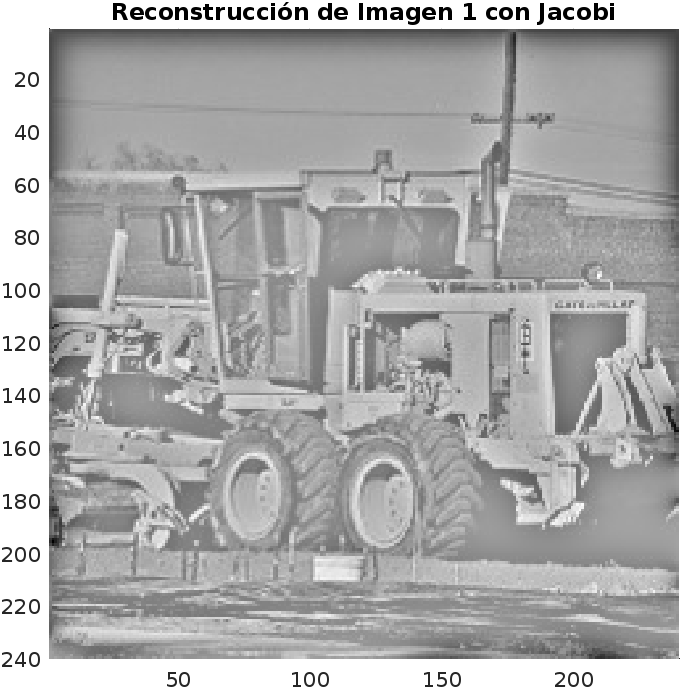
\includegraphics[scale=1]{Figures/Figure_1J.png}
        \end{center}
        \newpage
      \item Imágen 1 (Gauss-Seidel) $\frac{1990}{49931}s=0.03985s$.
        \begin{lstlisting}[language = matlab]
format rational
%% Visualizar la solución
function visualizar(u, N, M, titulo)
    imagen = reshape(u, [N, M]); % Volver a forma de matriz
    figure;
    surf(imagen), shading flat, axis ij, axis equal, view(2);
    colormap gray;
    title(titulo);
end

%% Cargar datos de los bordes
data1 = load('bordes1.mat'); % Cargar archivo

f = data1.bordes1; % Extraer matriz de bordes

[N, M] = size(f); % Dimensiones de la imagen 1


%% Métodos Iterativos

% Inicialización de la solución
u = zeros(M,N); % x0 inicial
iteraciones = 0;

tic;
while (100 >= iteraciones)
    u_anterior = u;
    for i=2:M-1
        for j=2:N-1
            u(i, j) = (1/4) * (-f(i, j) + u(i-1, j) + u_anterior(i+1, j) + u(i, j-1) + u_anterior(i, j+1));
        end
    end
    iteraciones = iteraciones + 1;
end

tiempo = toc;
disp("Tiempo tomado en el método de Gauss-Seidel");
disp(tiempo);
visualizar(u, N, M, 'Reconstrucción de Imagen 1 con Gauss-Seidel'); 
        \end{lstlisting}
        \begin{center}
          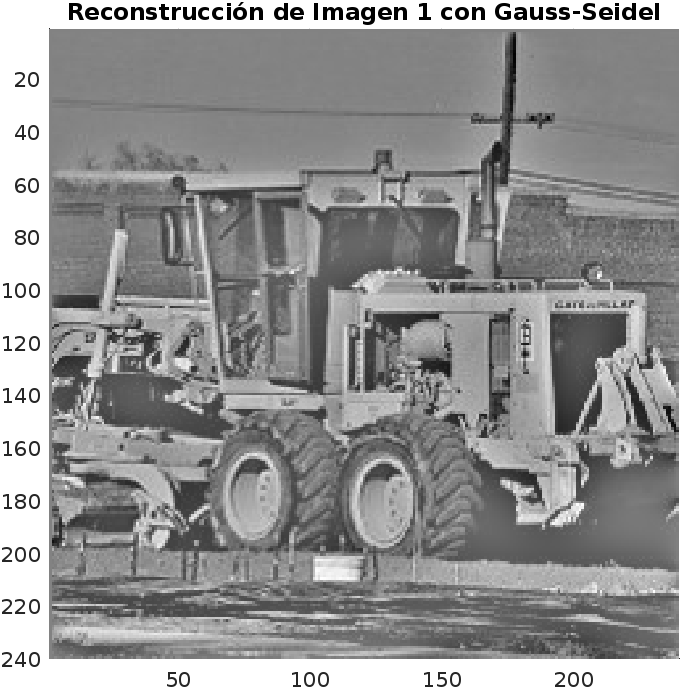
\includegraphics[scale=1]{Figures/Figure_1GS.png}
        \end{center}
        \newpage
      \item Imágen 1 (SOR) $\frac{396}{5729}s\approx 0.06912s$.
        \begin{lstlisting}[language = matlab]
format rational
%% Visualizar la solución
function visualizar(u, N, M, titulo)
    imagen = reshape(u, [N, M]); % Volver a forma de matriz
    figure;
    surf(imagen), shading flat, axis ij, axis equal, view(2);
    colormap gray;
    title(titulo);
end

%% Cargar datos de los bordes
data1 = load('bordes1.mat'); % Cargar archivo

f = data1.bordes1; % Extraer matriz de bordes
w = 1.5;
[N, M] = size(f); % Dimensiones de la imagen 1


%% Métodos Iterativos

% Inicialización de la solución
u = zeros(M,N); % x0 inicial
ugs = zeros(M,N);
iteraciones = 0;

tic;
while (100 >= iteraciones)
    u_anterior = u;
    for i=2:M-1
        for j=2:N-1
            ugs(i, j) = (1/4) * (-f(i, j) + u(i-1, j) + u_anterior(i+1, j) + u(i, j-1) + u_anterior(i, j+1));
            u(i, j) = (1-w)*u(i,j)+w*ugs(i,j);
        end
    end
    iteraciones = iteraciones + 1;
end

tiempo = toc;
disp("Tiempo tomado en el método de SOR con w=1.5");
disp(tiempo);
visualizar(u, N, M, 'Reconstrucción de Imagen 1 con SOR (w=1.5)');
        \end{lstlisting}
        \begin{center}
          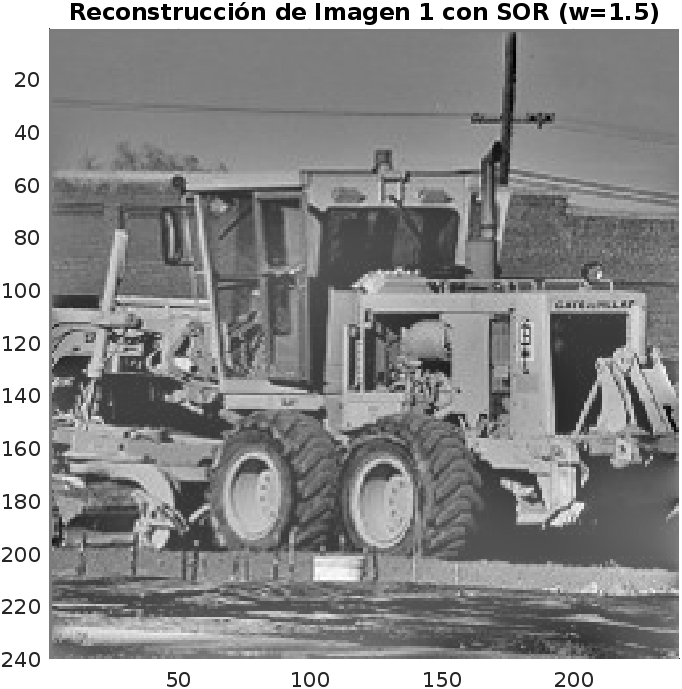
\includegraphics[scale=1]{Figures/Figure_1SOR.png}
        \end{center}
        \newpage
      \item Imágen 2 (Jacobi) $\frac{101}{2697}s\approx 0.03745s$.
        \begin{lstlisting}[language = matlab]
format rational
%% Construcción de la matriz A usando diferencias finitas
function A = construir_matriz_A(N, M)
    num_pixeles = N * M;
    A = sparse(num_pixeles, num_pixeles); % Matriz dispersa

    for i = 1:N
        for j = 1:M
            k = (i-1) * M + j; % Índice en el vector

            A(k, k) = -4; % Píxel central

            if j < M  % Vecino derecho
                A(k, k + 1) = 1;
            end
            if j > 1  % Vecino izquierdo
                A(k, k - 1) = 1;
            end
            if i < N  % Vecino inferior
                A(k, k + M) = 1;
            end
            if i > 1  % Vecino superior
                A(k, k - M) = 1;
            end
        end
    end
end

%% Visualizar la solución
function visualizar(u, N, M, titulo)
    imagen = reshape(u, [N, M]); % Volver a forma de matriz
    figure;
    surf(imagen), shading flat, axis ij, axis equal, view(2);
    colormap gray;
    title(titulo);
end

%% Cargar datos de los bordes
data2 = load('bordes2.mat'); % Cargar archivo

f = data2.bordes2; % Extraer matriz de bordes

[N, M] = size(f); % Dimensiones de la imagen 2

% Convertir la matriz en un vector columna
f_vec = f(:);

A = construir_matriz_A(N, M);

%% Métodos Iterativos

D = diag(diag(A)); % Matriz diagonal
L = -tril(A,-1);   % Parte triangular inferior estricta con signo negativo
U = -triu(A,1);    % Parte triangular superior estricta con signo negativo

% Jacobi

TJ = inv(D)*(U+L);
cJ = inv(D)*f_vec;
[f_size, basura] = size(f_vec);

u = zeros(f_size,1); % u0 inicial
u_anterior = u+1; % Para comparar iteraciones
iteraciones = 0;

% Iterar hasta que haga 100 iteraciones del método

tic;
while (100 >= iteraciones)
    u_anterior = u; % Guardar el u anterior
    u = TJ * u + cJ; % Nueva iteración
    iteraciones = iteraciones + 1;
end

tiempo = toc;

disp("Tiempo tomado en el método Jacobi:")
disp(tiempo);
visualizar(u, N, M, 'Reconstrucción de Imagen 2 con Jacobi');
        \end{lstlisting}
        \begin{center}
          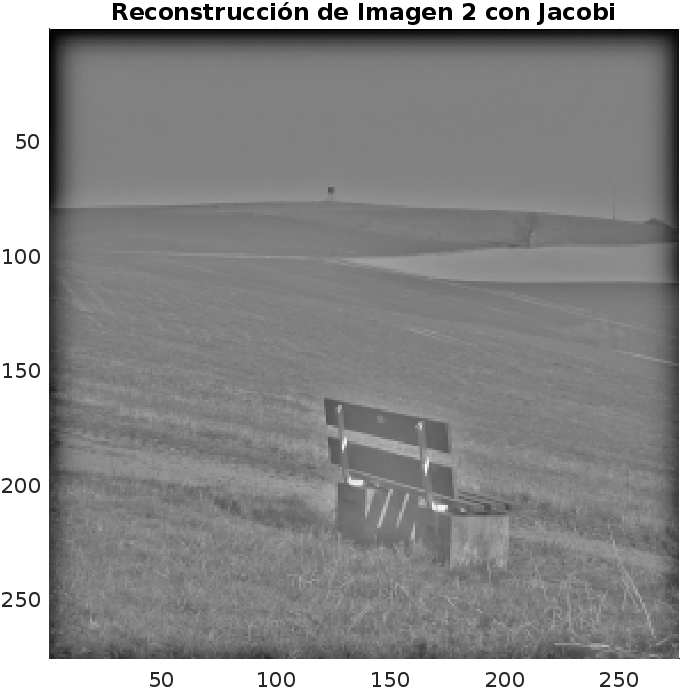
\includegraphics[scale=1]{Figures/Figure_2J.png}
        \end{center}
      \item Imágen 2 (Gauss-Seidel) $\frac{159}{2323}s=0.06845s$.
        \begin{lstlisting}[language = matlab]
format rational
%% Visualizar la solución
function visualizar(u, N, M, titulo)
    imagen = reshape(u, [N, M]); % Volver a forma de matriz
    figure;
    surf(imagen), shading flat, axis ij, axis equal, view(2);
    colormap gray;
    title(titulo);
end

%% Cargar datos de los bordes
data2 = load('bordes2.mat'); % Cargar archivo

f = data2.bordes2; % Extraer matriz de bordes

[N, M] = size(f); % Dimensiones de la imagen 2


%% Métodos Iterativos

% Inicialización de la solución
u = zeros(M,N); % x0 inicial
iteraciones = 0;

tic;
while (100 >= iteraciones)
    u_anterior = u;
    for i=2:M-1
        for j=2:N-1
            u(i, j) = (1/4) * (-f(i, j) + u(i-1, j) + u_anterior(i+1, j) + u(i, j-1) + u_anterior(i, j+1));
        end
    end
    iteraciones = iteraciones + 1;
end

tiempo = toc;
disp("Tiempo tomado en el método de Gauss-Seidel");
disp(tiempo);
visualizar(u, N, M, 'Reconstrucción de Imagen 2 con Gauss-Seidel');
        \end{lstlisting}
        \begin{center}
          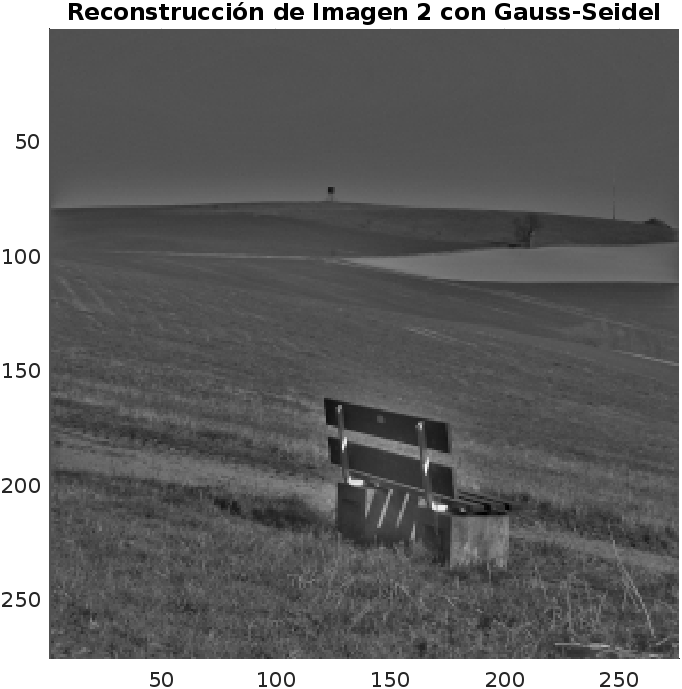
\includegraphics[scale=1]{Figures/Figure_2GS.png}
        \end{center}
        \newpage
      \item Imágen 2 (SOR) $\frac{163}{2617}s \approx 0.06229s$.
        \begin{lstlisting}[language = matlab]
format rational
%% Visualizar la solución
function visualizar(u, N, M, titulo)
    imagen = reshape(u, [N, M]); % Volver a forma de matriz
    figure;
    surf(imagen), shading flat, axis ij, axis equal, view(2);
    colormap gray;
    title(titulo);
end

%% Cargar datos de los bordes
data2 = load('bordes2.mat'); % Cargar archivo

f = data2.bordes2; % Extraer matriz de bordes
w = 1.5;
[N, M] = size(f); % Dimensiones de la imagen 2


%% Métodos Iterativos

% Inicialización de la solución
u = zeros(M,N); % x0 inicial
ugs = zeros(M,N);
iteraciones = 0;

tic;
while (100 >= iteraciones)
    u_anterior = u;
    for i=2:M-1
        for j=2:N-1
            ugs(i, j) = (1/4) * (-f(i, j) + u(i-1, j) + u_anterior(i+1, j) + u(i, j-1) + u_anterior(i, j+1));
            u(i, j) = (1-w)*u(i,j)+w*ugs(i,j);
        end
    end
    iteraciones = iteraciones + 1;
end

tiempo = toc;
disp("Tiempo tomado en el método de SOR con w=1.5");
disp(tiempo);
visualizar(u, N, M, 'Reconstrucción de Imagen 2 con SOR (w=1.5)');
        \end{lstlisting}
        \begin{center}
          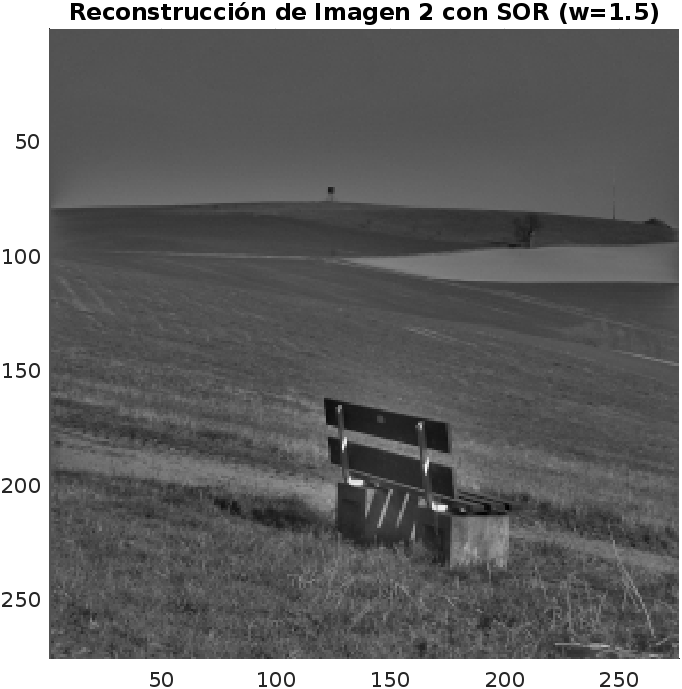
\includegraphics[scale=1]{Figures/Figure_2SOR.png}
        \end{center}
        \newpage
    \end{enumerate}
    \textbf{Comparación:}
    \begin{center}
      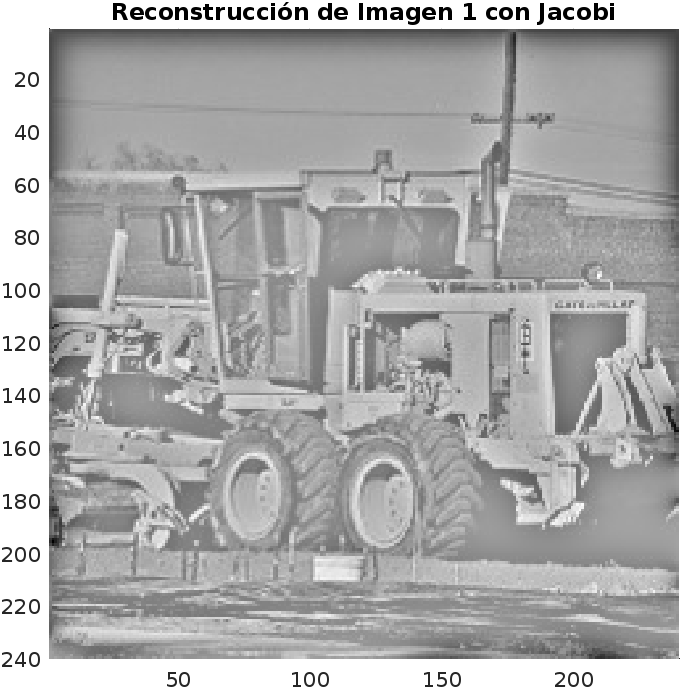
\includegraphics[scale=0.6]{Figures/Figure_1J.png}
      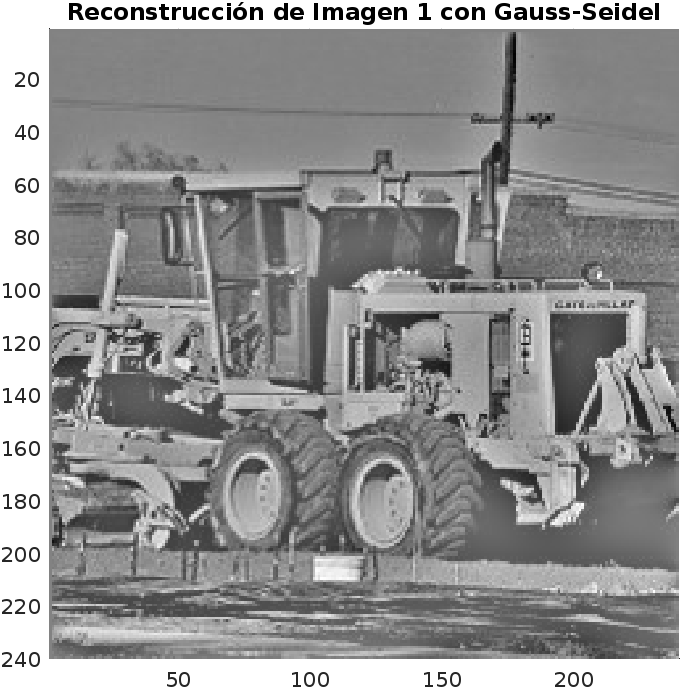
\includegraphics[scale=0.6]{Figures/Figure_1GS.png}
      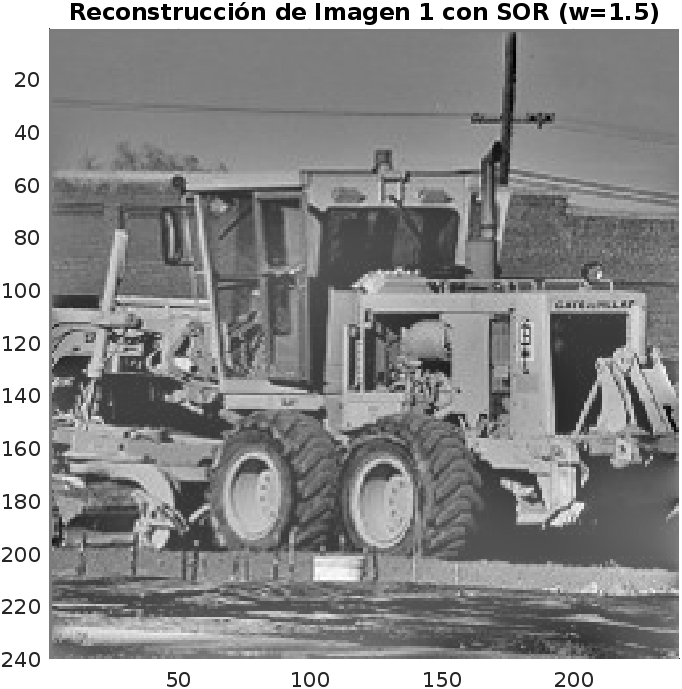
\includegraphics[scale=0.6]{Figures/Figure_1SOR.png}
      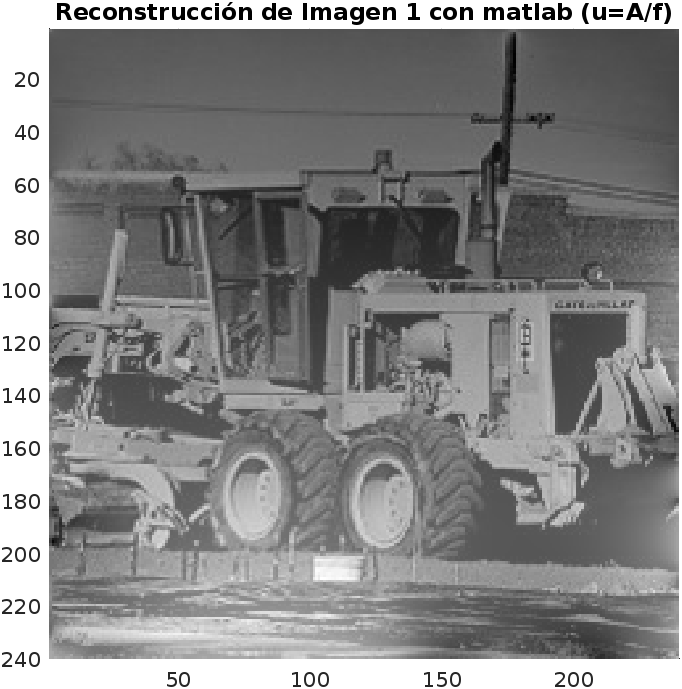
\includegraphics[scale=0.6]{Figures/Figure_1matlab.png}\\
    \end{center}
    \begin{center}
      \begin{tabular}{|c|c|}
        \hline
        Método & Tiempo (s)\\
        \hline
        Jacobi & 0,0304\\
        \hline
        Gauss-Seidel & 0,0398\\
        \hline
        SOR & 0,0691\\
        \hline
      \end{tabular}        
    \end{center}
    \begin{center}
      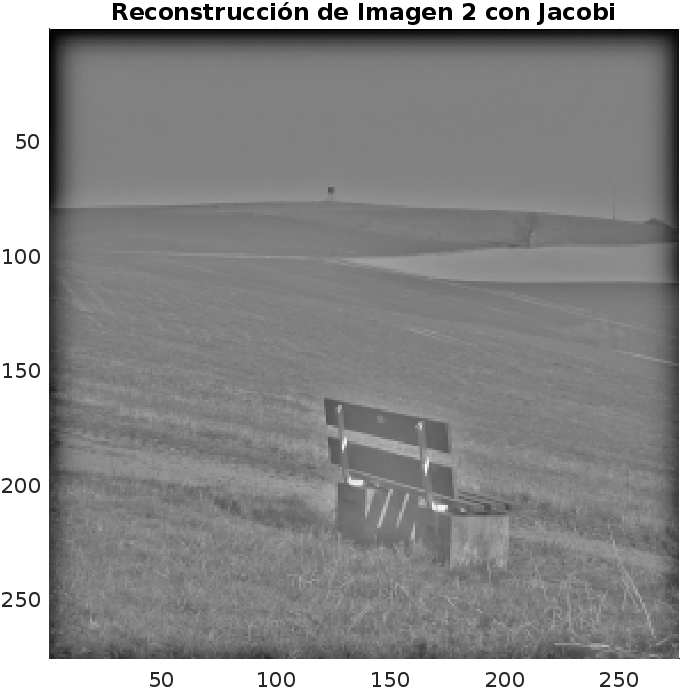
\includegraphics[scale=0.6]{Figures/Figure_2J.png}
      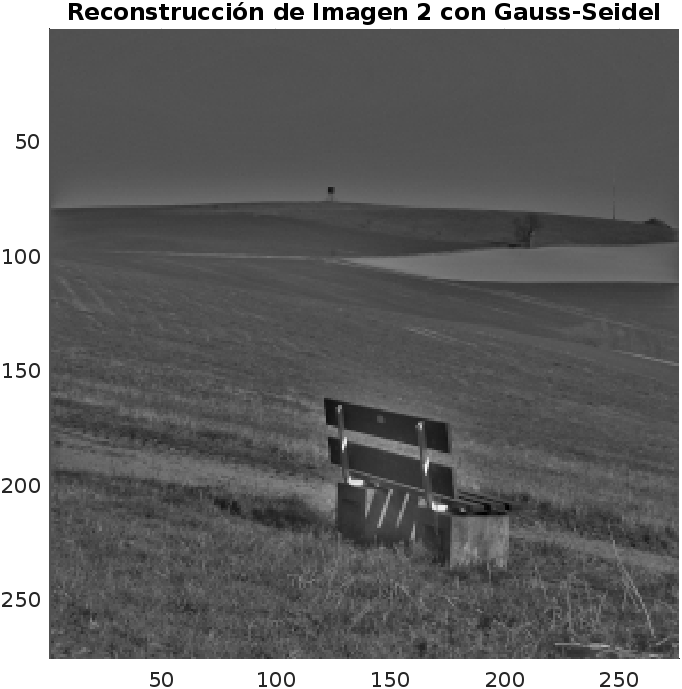
\includegraphics[scale=0.6]{Figures/Figure_2GS.png}
      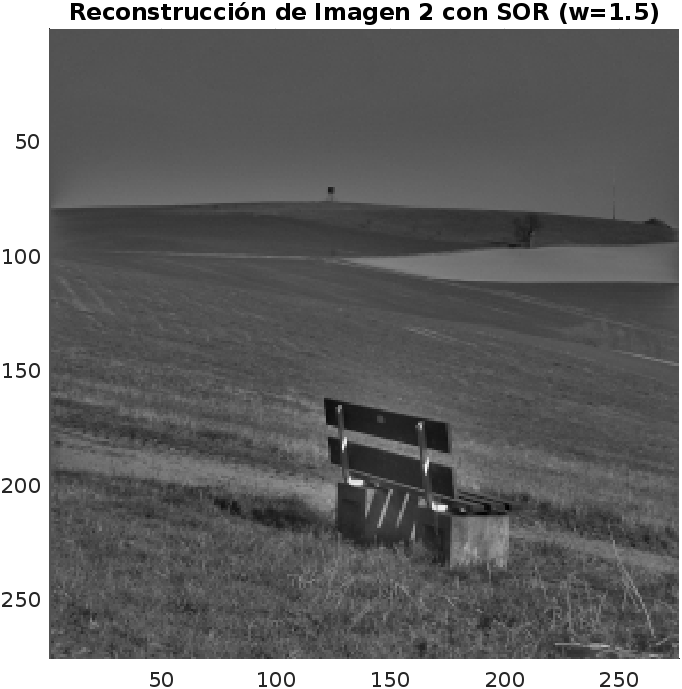
\includegraphics[scale=0.6]{Figures/Figure_2SOR.png}
      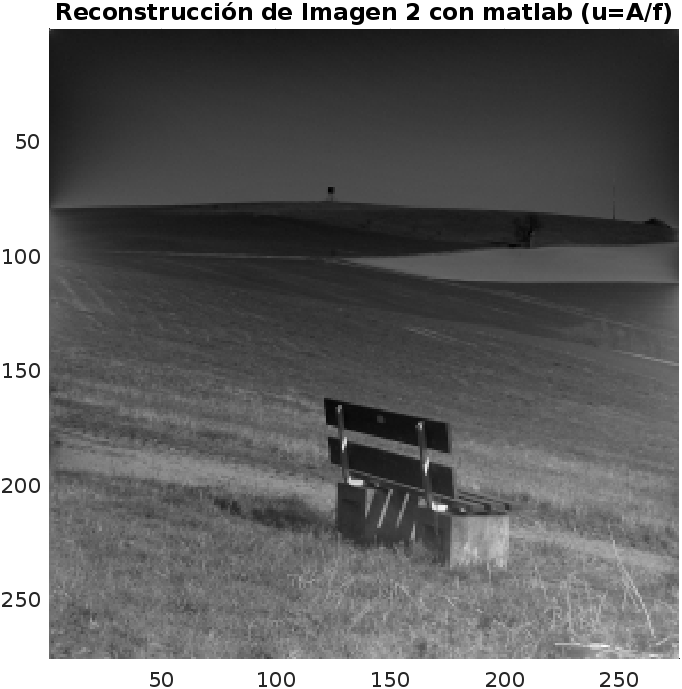
\includegraphics[scale=0.6]{Figures/Figure_2matlab.png}
    \end{center}
    \begin{center}
      \begin{tabular}{|c|c|}
        \hline
        Método & Tiempo (s)\\
        \hline
        Jacobi & 0,0374\\
        \hline
        Gauss-Seidel & 0,0685\\
        \hline
        SOR & 0,0623\\
        \hline
      \end{tabular}        
    \end{center}
    \textbf{Conclusiones:} con esto podemos llegar experimentalmente a que "aparentemente" el método de $SOR$ es más efectivo que Jacobu y Gauss-Seidel, por lo que en las mismas 100 iteraciones logró obtener mejores resultados, no obstante, hay que considerar que en el ejercicio el método de Jacobi tardó menos tiempo en ambas imágenes, por lo que se podría pensar que quizás comparandolas por tiempo se podría llegar a otras conclusiones. Por otro lado, hay que contar con las modificaciones que se tuvieron que hacer para poder lograr hacer óptima la aplicación de los métodos de Gauss-Seidel y SOR en matlab (situación que comentamos en la nota), por lo que quizás si realizaramos el mismo trato en Jacobi podrían cambiar las situaciones.\\
    No obstante, es claro que SOR logró un mejor resultado y que en las primeras $100$ iteraciones ese tiempo entre él y los demás es prácticamente despreciable en pro de que $SOR$ realizó la tarea de una forma más efectiva. 
  \end{solucion}
\end{homeworkProblem}
